%%%%%%%%%%%%%%%%%%%%%%%%%%%%%%%%%%%%%%%%%
% Short Three-Column Newsletter
% LaTeX Template
% Version 1.0 (11/9/13)
%
% Original author:
% Frits Wenneker (http://www.howtotex.com) 
% With extensive modifications by:
% Vel (vel@latextemplates.com)
% 
% This template has been downloaded from:
% http://www.LaTeXTemplates.com
%
% License:
% CC BY-NC-SA 3.0 (http://creativecommons.org/licenses/by-nc-sa/3.0/)
%
%%%%%%%%%%%%%%%%%%%%%%%%%%%%%%%%%%%%%%%%%

%----------------------------------------------------------------------------------------
%	PACKAGES AND DOCUMENT CONFIGURATIONS
%----------------------------------------------------------------------------------------

\documentclass[10pt,a4paper]{article} % Paper type (a4paper, usletter or legal) and font size (10, 11 or 12)

\setlength\topmargin{-48pt} % Top margin
\setlength\headheight{0pt} % Header height
\setlength\textwidth{7.0in} % Text width
\setlength\textheight{9.5in} % Text height
\setlength\oddsidemargin{-30pt} % Left margin
\setlength\evensidemargin{-30pt} % Left margin (even pages) - only relevant with 'twoside' article option

\usepackage{charter} % Charter font for main content
\usepackage{siunitx}
\frenchspacing % Reduces space after periods to make text more compact for a three-column layout

\usepackage{graphicx} % Required for including images
\usepackage{amssymb,amsmath} % Math packages
\usepackage{multicol} % Required for the three-column layout of the document
\usepackage{url} % Clickable links
\usepackage{enumitem} % Reduces the amount of space within and between lists with [noitemsep,nolistsep]
\usepackage{marvosym} % Required for the use of symbols
\usepackage{wrapfig} % Allows wrapping text around figures
\usepackage[T1]{fontenc} % Use 8-bit encoding that has 256 glyphs
\usepackage{datetime} % Required for defining a custom date style
\newdateformat{mydate}{\monthname[\THEMONTH] \THEYEAR} % Set a custom date format
\usepackage[pdfpagemode=FullScreen, colorlinks=false]{hyperref} % Link colors and PDF behavior in Acrobat
\usepackage{fancyhdr} % Required to define custom headers/footers
\pagestyle{fancy} % Enables the custom headers/footers for all pages following this

%-----------------------------------------------------------
% Header and footer
\lfoot{\footnotesize % Left footer containing newsletter contact information
	Studying in four different countries during my Master Degree\\
	\Mundus\ \href{https://github.com/stefanos1316/my_blog/index.com}{my\_blog/index.com} \quad
	%\Telefon\ Not available yet \quad
	\Letter\ \href{mailto:sgeorgiou@aueb.gr}{sgeorgiou@aueb.gr}
}


\cfoot{} % Empty center footer

\rfoot{\footnotesize ~\\ Page \thepage} % Right footer - page counter

\renewcommand{\headrulewidth}{0.0pt} % No horizontal rule for the header
\renewcommand{\footrulewidth}{0.4pt} % Horizontal rule separating the footer from the document
%-----------------------------------------------------------

%-----------------------------------------------------------
% Define separators
\newcommand{\HorRule}[1]{\noindent\rule{\linewidth}{#1}} % Creates a horizontal rule
\newcommand{\SepRule}{\noindent	% Creates a shorter separator rule
\begin{center}
\rule{250pt}{1pt} % Page width and rule width
\end{center}
}
%-----------------------------------------------------------

%-----------------------------------------------------------
% Define title and article styles
\newcommand{\NewsletterName}[1]{ % Newsletter title
\begin{center}
\Huge \usefont{T1}{fvs}{b}{n} % Use the Bera Sans Bold font
#1
\end{center}	
\par \normalsize \normalfont}

\newcommand{\JournalIssue}[1]{ % Date and issue number at the top of the newsletter
\hfill \textsc{\mydate \today, No #1} % Right-aligned date and issue number
\par \normalsize \normalfont}

\newcommand{\NewsItem}[1]{ % News item title
\usefont{T1}{fvs}{n}{n} % Use the Bera Sans Normal font
\vspace{24pt}\large #1\vspace{3pt} % Print the title with space around it in a larger font size
\par \normalsize \normalfont}

\newcommand{\NewsAuthor}[1]{ % Author name under the item title
\hfill by \textsc{#1} \vspace{20pt} % Right-aligned author name in small caps with space after it
\par \normalfont}		

%----------------------------------------------------------------------------------------
%	TITLE
%----------------------------------------------------------------------------------------

\begin{document}

\JournalIssue{1} % Issue number

\NewsletterName{Studying in four different countries} % Newsletter title

\noindent\HorRule{3pt} \\[-0.75\baselineskip] % Thick horizontal rule
\HorRule{1pt} % Thin horizontal rule

%----------------------------------------------------------------------------------------
%	MAIN NEWS ITEM
%----------------------------------------------------------------------------------------

\vspace{0.5cm}
\SepRule
\vspace{-0.5cm}

\begin{center}
\begin{minipage}[h]{0.75\linewidth}
\begin{wrapfigure}{l}{0.45\textwidth}
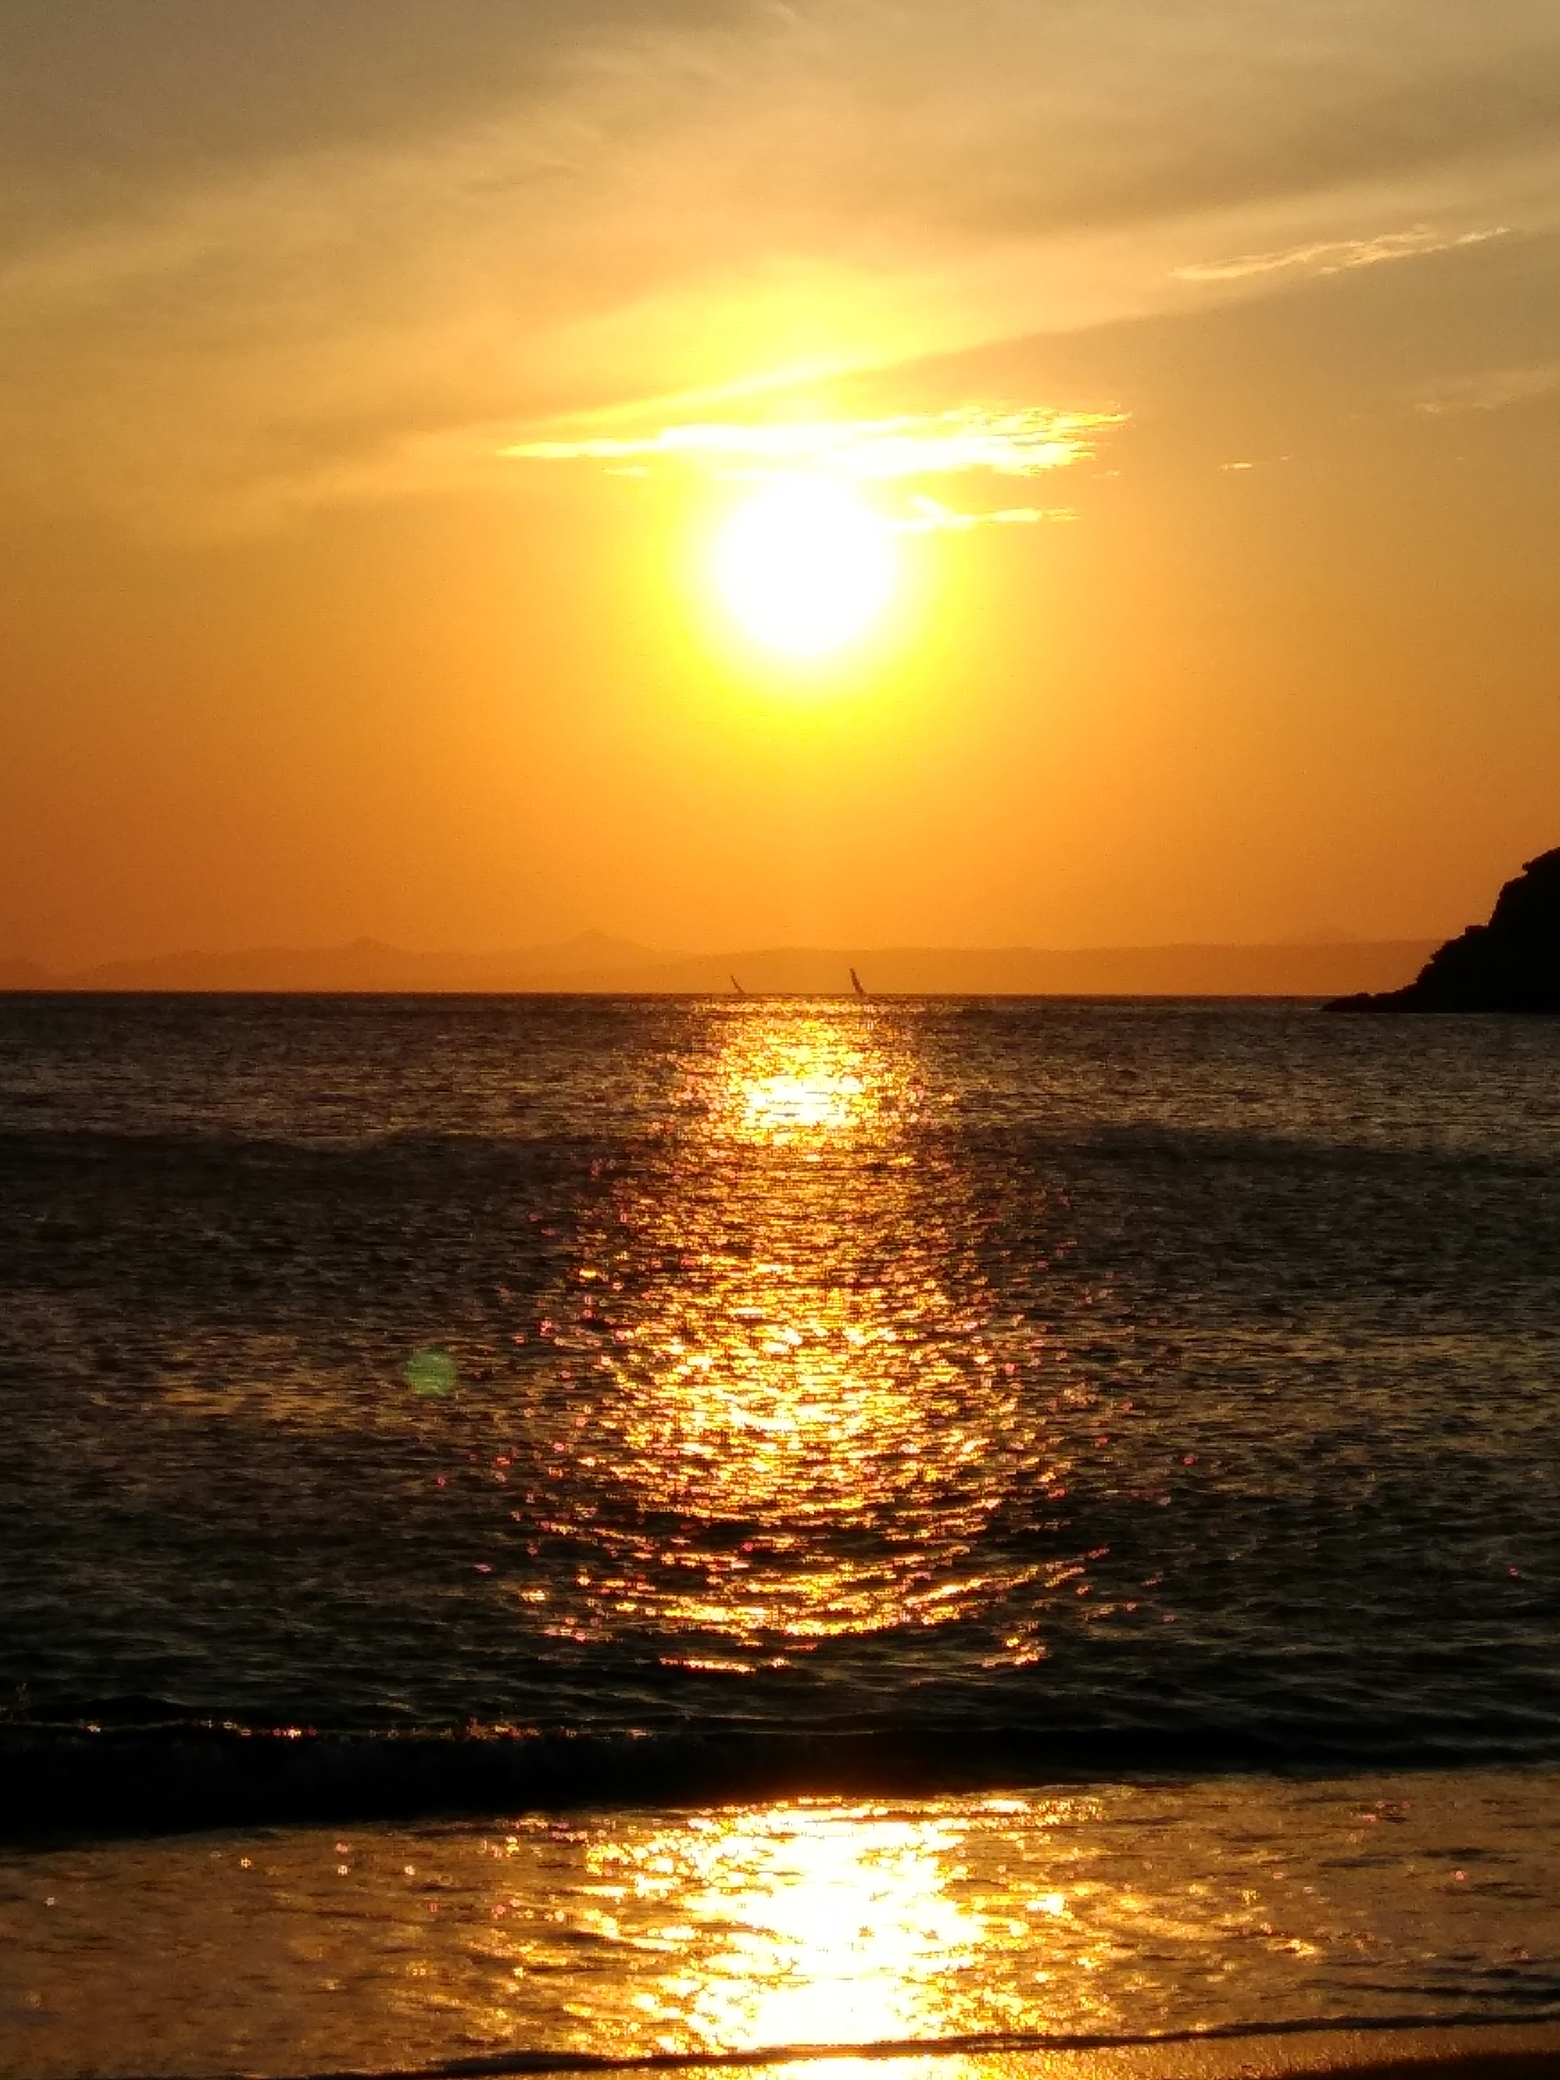
\includegraphics[width=0.45 \textwidth]{media/front_picture.jpg}
\\
\end{wrapfigure}
	
\NewsItem{Author's thoughts} % Main next item title
\vspace{3pt} % Some extra whitespace since there is no author as for the news in the body of the newsletter
\textit{
%12345678901234567890123456789012345678901234567890123456789012345678901234567890
An extortionary beauty, simplicity, relaxation can be found in the islands of Greece. 
}
\par\hfill --- Stefanos Georgiou
\end{minipage}
\end{center}

\vspace{0.5cm}
\SepRule % Small horizontal rule after the main news item
\vspace{0.5cm}

%\setlength{\columnsep}{16pt} % Uncomment to manually change the white space between columns
\begin{multicols}{3} % Begin the three-column layout

%----------------------------------------------------------------------------------------
%	OTHER NEWS
%----------------------------------------------------------------------------------------

\NewsItem{What was I thinking?}
\NewsAuthor{Stefanos Georgiou}

%12345678901234567890123456789012345678901234567890123456789012345678901234567890
% We are going to discuss about greek islands 
% Discuss interesting stories such as Tzia and the almost dry out from water
% Discuss the Milos trip with Ana Kalisnik
% Discuss about Chania and the driving with Alexandre De Masi.
% Discuss about Salamina and how much Antonis still mentioning the kotsi
% Discuss about Hydra and how Dorine was saying...can we not go back to Athens and stay here?
% Discuss about Aigina with Andreas Tattis
% Discuss about Agkistri with Fisayo.
% Discuss about Leukada with Voijak.


\begin{center}
	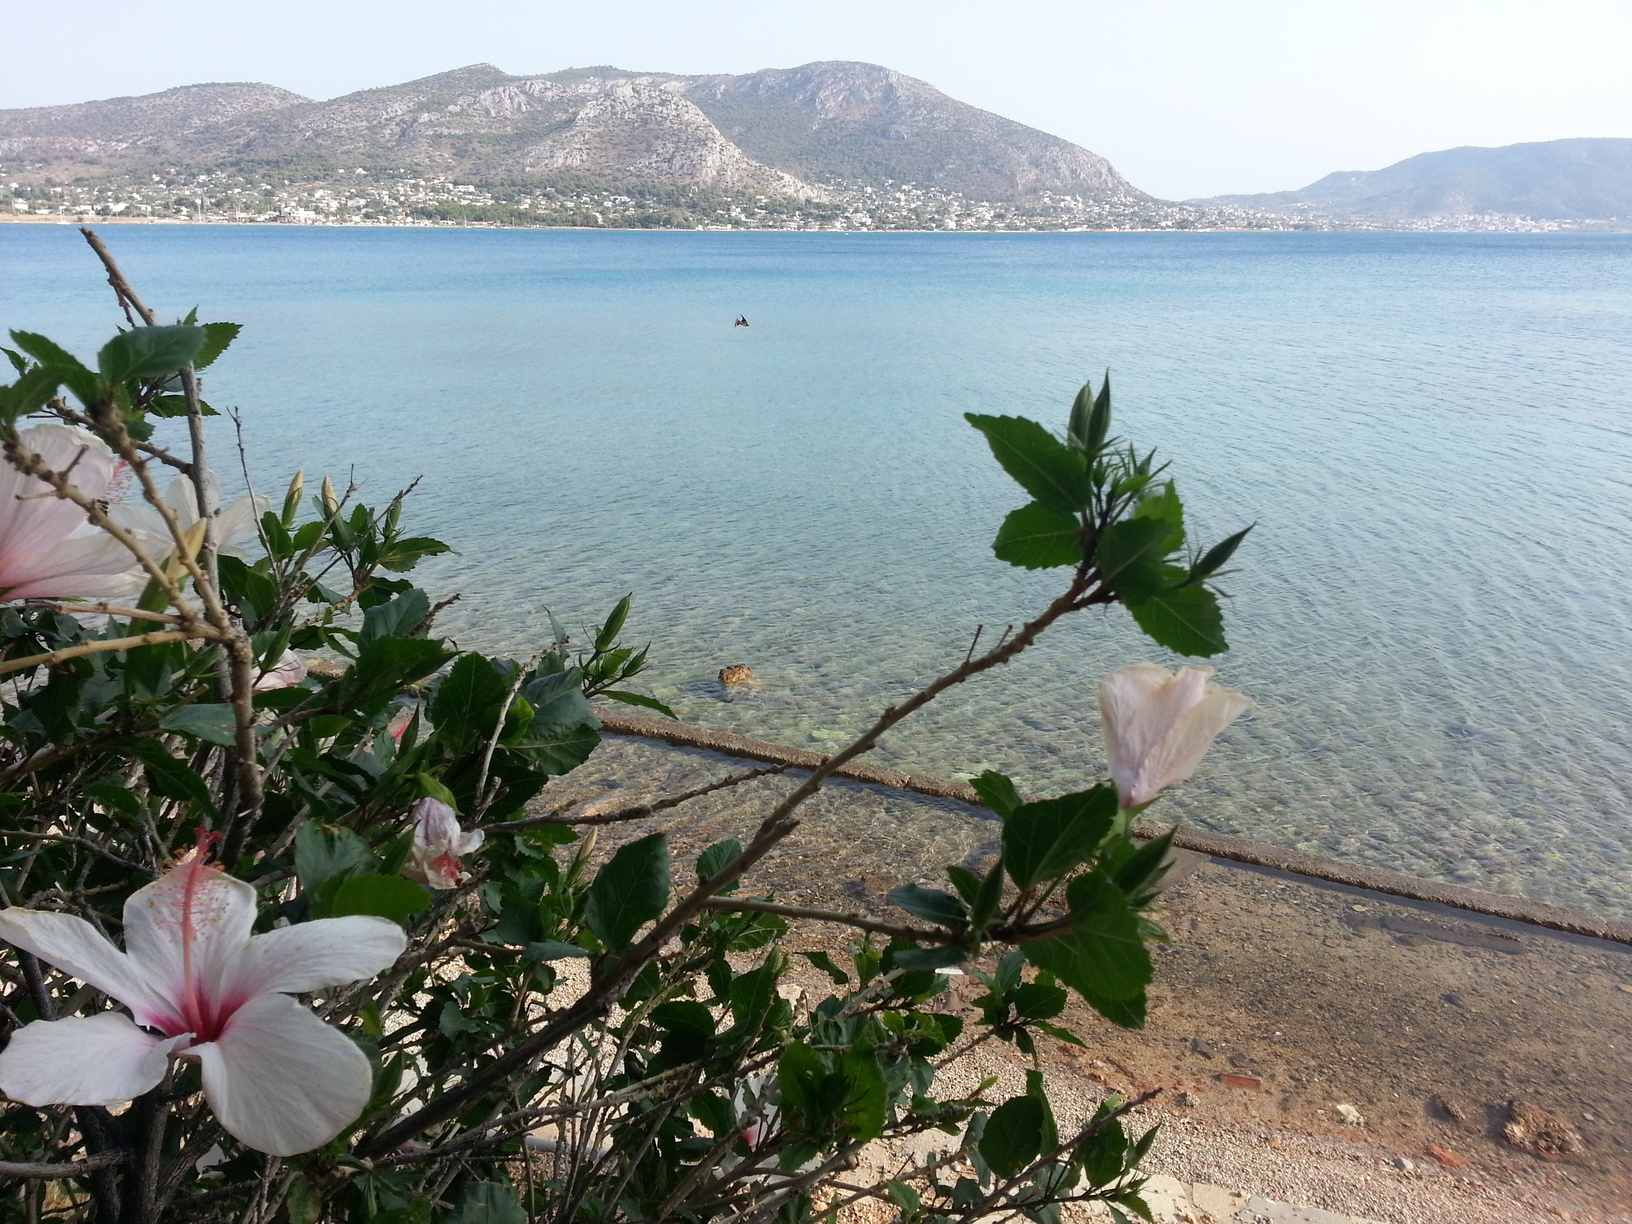
\includegraphics[width=0.32\textwidth]{media/salamina_1.jpg}
	\par\textit{The island of Salamina}
\end{center}


\end{multicols}



%----------------------------------------------------------------------------------------



\end{document} 